
\medskip

Dans cet exercice, on va s'intéresser à la vitesse d'un TGV passant en gare sans s'arrêter.

\medskip

Information 1 :  Tout le train est passé devant moi en 13 secondes et 53 centièmes.

\medskip

Information 2 : Schéma des motrices et voitures composant une rame de TGV :

\begin{center}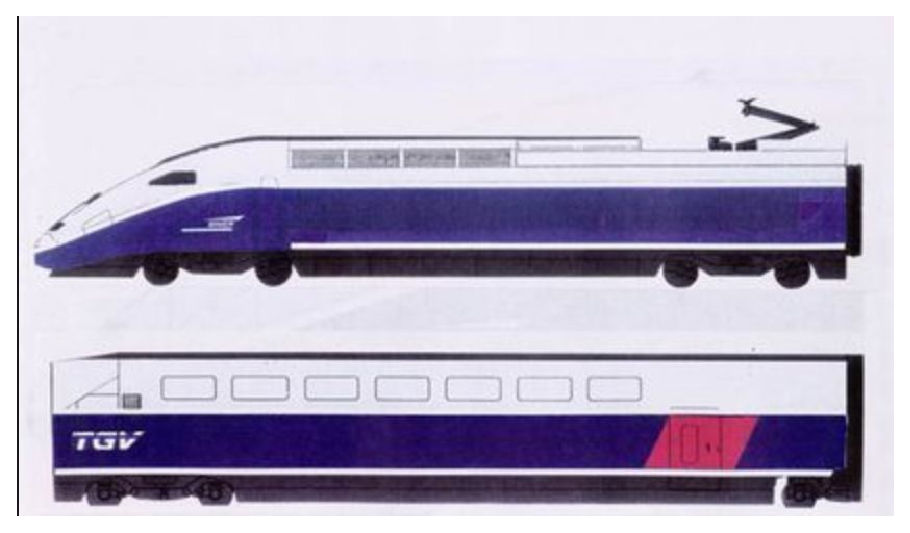
\includegraphics[width=10cm]{rameTGV.eps}
\hspace{-10cm}
\begin{pspicture}(10,5)
\psline{<->}(0.1,2.4)(2,2.4)\uput[d](1.05,2.4){\np{5000}}
\psline{<->}(2,2.4)(9.5,2.4)\uput[d](5.75,2.4){\np{14000}}
\psline{<->}(0.25,-0.4)(9.5,-0.4)\uput[u](4.975,-0.4){\np{18300}}
\rput(10.5,3){A. motrice}
\rput(10.5,1){B. voiture}
\end{pspicture}
\end{center}

\bigskip

Les mesures de longueur sont exprimées en millimètre

\medskip

Information 3 : Composition du TGV passé en gare :

\setlength\parindent{9mm}
\begin{tabularx}{\linewidth}{|X|}\hline
\begin{itemize}
\item[$\bullet~~$] Le TGV est constitué de deux rames.
\item[$\bullet~~$] Chaque rame est composée de deux motrices de type A encadrant dix
voitures de type B.
\end{itemize}\\ \hline
\end{tabularx}
\setlength\parindent{0mm} 

\smallskip
 
À quelle vitesse (en km/h) le TGV est-il passé, sans s'arrêter, devant moi ?
 
Le résultat sera arrondi à l'unité.

\bigskip

